\chapter{Proof of Concept}

\section{Szenario 1}\label{poc:scenario1}
\begin{comment}
\begin{figure}[htb]
    \begin{subfigure}[b]{0.5\columnwidth}
      \includegraphics[width=\columnwidth]{fig/render_läuferverband50.png}
      \caption{Bla.}
      \label{fig:poc:render_läuferverband50}
    \end{subfigure}
    \hfill
    \begin{subfigure}[b]{0.5\columnwidth}
      \includegraphics[width=\columnwidth]{fig/render_crossbond.png}
      \caption{Bla.}
      \label{fig:poc:render_crossbond}
    \end{subfigure}
    \begin{subfigure}[b]{0.5\columnwidth}
      \includegraphics[width=\columnwidth]{fig/render_headbond.png}
      \caption{Bla.}
      \label{fig:poc:render_headbond}
    \end{subfigure}
    \caption{Ergebnisse.}
    \label{fig:poc:result_scenario1}
  \end{figure}
\end{comment}

\section{Szenario 2}
\begin{figure}[hb]
  \centering
  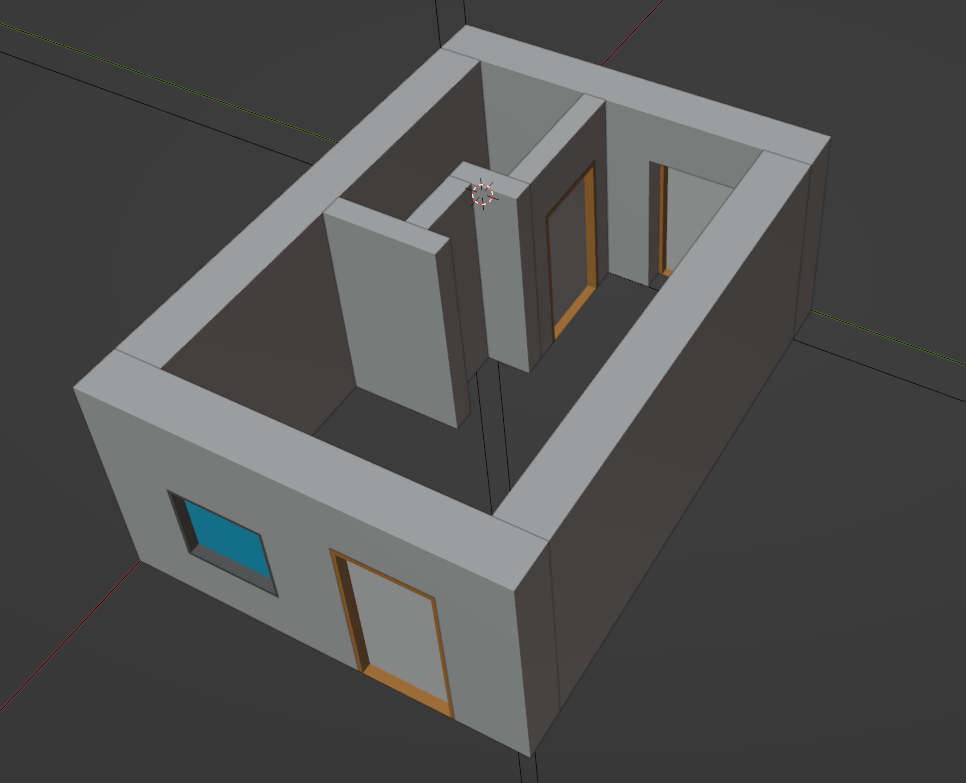
\includegraphics[width=0.5\columnwidth]{fig/scenario1_screenshot.png}
  \caption{3D Modell innerhalb von Blender.}
  \label{fig:poc:Scenario1 Screenshot}
\end{figure}